\chapter{序論}


\section{緒論}
%緒論,,どのくらいかくのかな
\clearpage
%2ページとか??4ページとか??


%\begin{figure}[tb]\centering
%\epsfxsize=10cm\epsffile{eps/nattorice.eps}
%\caption{元気の源,納豆ごはん}\label{fig:nattorice}
%\end{figure}

近年スマートデバイスの普及・通信技術の発達により,個人が各自端末を持ち歩くようになった.
このようなデバイスには,通信機能や音声入力・出力装置など様々なセンサやアクチュエータが搭載されており,デバイスを保持しているユーザに様々なサービスを提供できる.
近年はユビキタスな情報サービスとして各端末から情報を集め多数のユーザへのサービス状態を最適化するための研究もある.
このように,多人数からのリソースと取得データを用いた多人数へのサービスが実現できるようになった.

- Yu Zheng, Yanchi Liu, Jing Yuan, and Xing Xie, Urban Computing with Taxicabs, In Proc. of Ubicomp 2011, pp. 89--98, 2011.

実空間内のユーザ間でのコミュニケーション引き起こすものとして,すれ違い通信のような個人と個人の関係性に着目したものがあるが,多くの人が存在する空間の中で多人数のコミュニケーションに着目したものは見られない.

- 末廣 創,佐藤 文明,すれ違い通信による情報伝搬モデルの特性評価,情報処理学会全国大会講演論文集 第72回(ネットワーク), 155-156, 2010-03-08, 2010.

本研究では,授業や講演,学会発表などのある程度大規模な閉鎖空間での,一人対多人数のコミュニケーションに注目した.
これまでのような話し手が一方的に聴衆に話し続けるだけのコミュニケーションではなく,疑問や未理解・不明点といった反応を,話し手および聴衆の双方に即時的にフィードバックすることで,不明点の質問に臆することが減ったり,重要個所の情報を強調的に取得出来たりするなど,よりアクティブな知的コミュニケーション空間を作ることができると考えた.

これまでにもclickerやリアルタイムアンケートシステム,twitterやchat画面への書き込みによる,講義へのフィードバック手法が試みられている.
しかしこれらは視覚的情報でのフィードバックが多いため,講演や講義などの話者が中断することなくその内容を知ることはできず,結果として参加者からの意見が必須なシーンのみ活用されたり,参加者同士のコミュニケーションのみを盛り上げることになる.

- April R. Trees, and Michele H. Jackson. The learning environment in clicker classrooms: student processes of learning and involvement in large university‐level courses using student response systems. Learning, Media and Technology, vol.32, no.1, pp.21--40, 2007.
- 株式会社天問堂, Imakiku, http://tenmondo.com/products/imakiku/index.html (2015時点)
- 後藤 真孝, WISS 2010 と WISS 2011 での改革, コンピュータソフトウェア (日本ソフトウェア科学会誌), Vol.29, No.4, pp.3--8, 2012.


\section{研究の目的}

それに対し本研究では,広い空間内にいる多人数の端末を用いた音声コミュニケーション手法として,音源定位を用いた同時多発的なやり取りを提案する.
そして,特殊な音響装置のある教室や講演スペースによらず実現するため,参加者個人の端末をスピーカアレイとして活用することを考えた.

%\begin{figure}[tb]\centering
%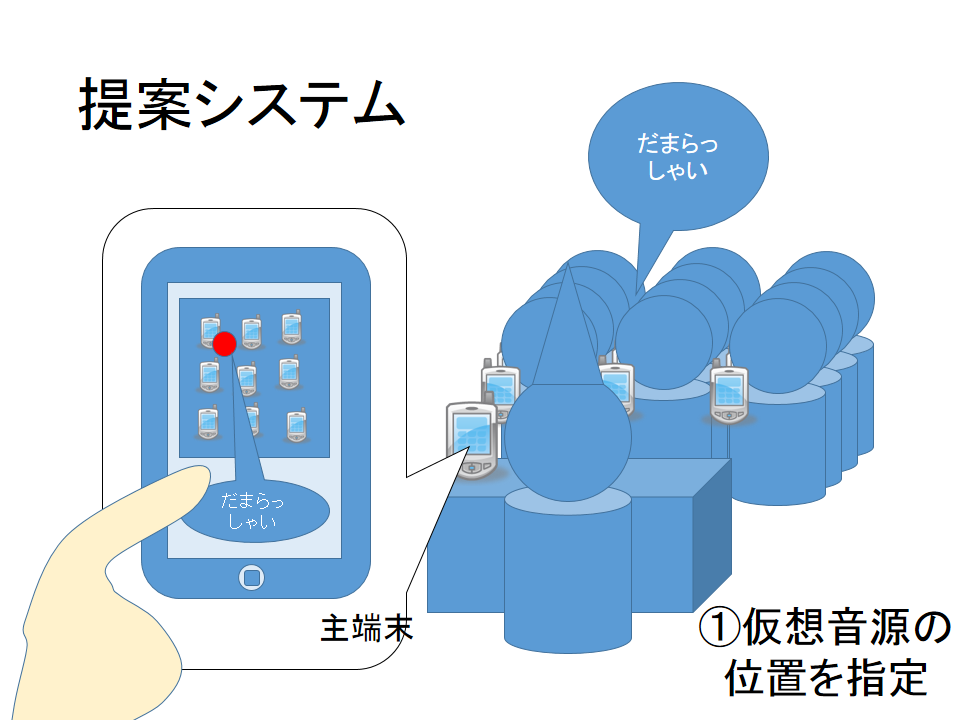
\includegraphics[clip,width=1.05\hsize]{../img/shikumi1.png}
%\caption{しくみ}\label{fig:shikumi1}
%\ecaption{Matched filter in transmission model}
%\end{figure}

本稿では,これらの端末が互いの位置や時間遅れを把握し,適切な音源定位による音声情報提示を行うため,端末間の距離測および同期手法として,
直接スペクトル拡散方式による測距手法を提案する.これにより,比較的高精度な同期と端末間の距離計測が行われる.音源定位を指定した音声情報提示の際には,端末間距離情報が,

1. どの端末を用いるか
2. どの程度の振幅パニングにより音源位置を設定するか

にそれぞれ用いられる.

これにより,特定多数のユーザによるパラレルコミュニケーションの実現だけでなく,駅構内や避難所などの不特定多数のユーザがいる空間においても,適切に音源定位した音声情報提示を行うことができるようになると期待される.



%ここはかなり大事
\clearpage
%わかりやすく,段落を丁寧に区切りましょう

\section{本論文の構成}
